% !TEX root = ../main.tex

%%%%%%%%%%%%%%%%%%%%%%%%%%%%%%%%%%%%%%%%%%%%%%%%%%%%%%%%%%%%%%%%%%%%%%%%%%%%%%%% 
%%% Appendix
%%%%%%%%%%%%%%%%%%%%%%%%%%%%%%%%%%%%%%%%%%%%%%%%%%%%%%%%%%%%%%%%%%%%%%%%%%%%%%%%

\chapter{Appendix}

\section{RSA}
\begin{Verbatim}[fontsize=\small]
binModExp(u32 base, u32 pow, u32 mod, u32 res){
    u32 tmp;
    res += 1;               
    for (i=32;0){           
       if ((1<<i)<=pow){
          square(res);        
          tmp += res%mod;     
          tmp <-> res;
          if (pow & (1<<i)){  
              res *= base;     
              tmp += res%mod;   
              tmp <-> res;
            }
        }
        i--;
     }
}

square(u32 x){
   x += 1;
}

main(){
    u32 x;
    scanf("%u32",x);
    square(x);
    printf("%u32",x);
}

encrypt(u32 msg, u32 e, u32 n){
    call binModExp(msg, e, n);
}

decrypt(u32 c, u32 d, u32 n){
    call binModExp(c, d, n);
}
\end{Verbatim}

\section{Elliptic Curve}



\begin{figure}[H]
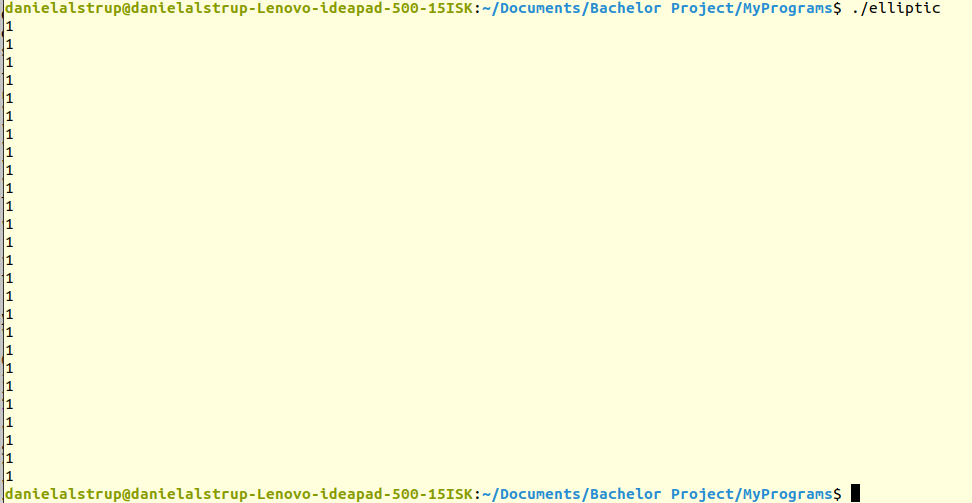
\includegraphics[width=0.9\textwidth]{figures/Tests}
\caption{Printout of a test-run.}
\label{fig:ECCTest}
\end{figure}


\begin{figure}[H]
  \begin{Verbatim}
runSign(){
  i32 p, a, verified;     
  i8 r, d;                
  i32 Q[2], G[2], R[2];  
  u32 msg[2],ver[2];
  // Set up curve, prime field, keys etc. 
  G[0] += 15;
  G[1] += 13;
  r += 10;               
  d += 13;               
  p += 17;

  call mult(G,Q,d,a,p);   
  call mult(G,R,r,a,p);   
  call readMsg(msg);
  ver[0] += msg[0];
  ver[1] += msg[1];

  //Signing.
  uncall decrypt(d,R,msg,a,p);
  // Message passed between users:
  // {Sign,uncall decrypt(Sign),R,r}
  uncall encrypt(Q,G,R,msg,r,a,p);
  
  if ((msg[0]==ver[0])&(msg[1]==ver[1])) verified += 1;
  
  // Write out the signature and a verification.
  printf("Signature verified: %i32\n",verified);
  call writeMsg(msg);
  call writeMsg(ver);
  
  uncall mult(G,Q,d,a,p);
  r -= 10;
  d -= 13;
  G[0] -= 15;
  G[1] -= 13;  
  p -= 17;
}
  \end{Verbatim}
\caption{A simple digital signature using asymmetric ECC.}
\label{fig:ECCSign}
\end{figure}

